%%%%%%%%%%%%%%%%%%%%%%%%%%%%%%%%%%%%%%%%%%%%%%
% An example of a lab report write-up.
%%%%%%%%%%%%%%%%%%%%%%%%%%%%%%%%%%%%%%%%%%%%%%
% This is a combination of several labs that I have done in the past for
% Computer Engineering, so it is not to be taken literally, but instead used as
% a great starting template for your own lab write up.  When creating this
% template, I tried to keep in mind all of the functions and functionality of
% LaTeX that I spent a lot of time researching and using in my lab reports and
% include them here so that it is fairly easy for students first learning LaTeX
% to jump on in and get immediate results.  However, I do assume that the
% person using this guide has already created at least a "Hello World" PDF
% document using LaTeX (which means it's installed and ready to go).
%
% My preference for developing in LaTeX is to use the LaTeX Plugin for gedit in
% Linux.  There are others for Mac and Windows as well (particularly MikTeX).
% Another excellent plugin is the Calc2LaTeX plugin for the OpenOffice suite.
% It makes it very easy to create a large table very quickly.
%
% Professors have different tastes for how they want the lab write-ups done, so
% check with the section layout for your class and create a template file for
% each class (my recommendation).
%
% Also, there is a list of common commands at the bottom of this document.  Use
% these as a quick reference.  If you'd like more, you can view the "LaTeX Cheat
% Sheet.pdf" included with this template material.
%
% (c) 2009 Derek R. Hildreth <derek@derekhildreth.com> http://www.derekhildreth.com
% This work is licensed under the Creative Commons Attribution-NonCommercial-ShareAlike License. To view a copy of this license, visit http://creativecommons.org/licenses/by-nc-sa/1.0/ or send a letter to Creative Commons, 559 Nathan Abbott Way, Stanford, California 94305, USA.
%%%%%%%%%%%%%%%%%%%%%%%%%%%%%%%%%%%%%%%%%%%%%%
\documentclass[aps,letterpaper,10pt]{revtex4}
\input kvmacros % For Karnaugh Maps (K-Maps)

\usepackage{graphicx} % For images
\usepackage{float}    % For tables and other floats
\usepackage{verbatim} % For comments and other
\usepackage{amsmath}  % For math
\usepackage{amssymb}  % For more math
\usepackage{fullpage} % Set margins and place page numbers at bottom center
\usepackage{listings} % For source code
\usepackage{subfig}   % For subfigures
\usepackage[usenames,dvipsnames]{color} % For colors and names
\usepackage[pdftex]{hyperref}           % For hyperlinks and indexing the PDF
\hypersetup{ % play with the different link colors here
    colorlinks,
    citecolor=blue,
    filecolor=blue,
    linkcolor=blue,
    urlcolor=blue % set to black to prevent printing blue links
}

\definecolor{mygrey}{gray}{.96} % Light Grey
\lstset{
	language=[ISO]C++,              % choose the language of the code ("language=Verilog" is popular as well)
   tabsize=3,							  % sets the size of the tabs in spaces (1 Tab is replaced with 3 spaces)
	basicstyle=\tiny,               % the size of the fonts that are used for the code
	numbers=left,                   % where to put the line-numbers
	numberstyle=\tiny,              % the size of the fonts that are used for the line-numbers
	stepnumber=2,                   % the step between two line-numbers. If it's 1 each line will be numbered
	numbersep=5pt,                  % how far the line-numbers are from the code
	backgroundcolor=\color{mygrey}, % choose the background color. You must add \usepackage{color}
	%showspaces=false,              % show spaces adding particular underscores
	%showstringspaces=false,        % underline spaces within strings
	%showtabs=false,                % show tabs within strings adding particular underscores
	frame=single,	                 % adds a frame around the code
	tabsize=3,	                    % sets default tabsize to 2 spaces
	captionpos=b,                   % sets the caption-position to bottom
	breaklines=true,                % sets automatic line breaking
	breakatwhitespace=false,        % sets if automatic breaks should only happen at whitespace
	%escapeinside={\%*}{*)},        % if you want to add a comment within your code
	commentstyle=\color{BrickRed}   % sets the comment style
}

% Make units a little nicer looking and faster to type
\newcommand{\Hz}{\textsl{Hz}}
\newcommand{\KHz}{\textsl{KHz}}
\newcommand{\MHz}{\textsl{MHz}}
\newcommand{\GHz}{\textsl{GHz}}
\newcommand{\ns}{\textsl{ns}}
\newcommand{\ms}{\textsl{ms}}
\newcommand{\s}{\textsl{s}}



% TITLE PAGE CONTENT %%%%%%%%%%%%%%%%%%%%%%%%
% Remember to fill this section out for each
% lab write-up.
%%%%%%%%%%%%%%%%%%%%%%%%%%%%%%%%%%%%%%%%%%%%%
\newcommand{\labno}{05}
\newcommand{\labtitle}{AI 3603 Artificial Intelligence: Principles and Techniques}
\newcommand{\authorname}{Zhao Xiangyu: 518021910982   Zhu Fuze: 519030910066}
\newcommand{\hw}{2}
% END TITLE PAGE CONTENT %%%%%%%%%%%%%%%%%%%%


\begin{document}  % START THE DOCUMENT!


% TITLE PAGE %%%%%%%%%%%%%%%%%%%%%%%%%%%%%%%%%%%%%%
% If you'd like to change the content of this,
% do it in the "TITLE PAGE CONTENT" directly above
% this message
%%%%%%%%%%%%%%%%%%%%%%%%%%%%%%%%%%%%%%%%%%%%%%%%%%%
\begin{titlepage}
\begin{center}
{\Large \textsc{\labtitle} \\ \vspace{4pt}}
\rule[13pt]{\textwidth}{1pt} \\ \vspace{150pt}
{\large By: \authorname \\ \vspace{10pt}
HW\#:\hw \\ \vspace{10pt}
\today}
\end{center}
\end{titlepage}
% END TITLE PAGE %%%%%%%%%%%%%%%%%%%%%%%%%%%%%%%%%%





%%%%%%%%%%%%%%%%%%%%%%%%%%%%%%
%%%%%%%%%%%%%%%%%%%%%%%%%%%%%%
\section{Introduction}
%No Text Here
%%%%%%%%%%%%%%%%%%%%%%%%%%%%%%%


In this assignment, we will implement Reinforcement Learning agents to find a safe path to the destination in a grid-shaped maze. The agent will learn by trail and error from interactions with the environment and finally acquire a policy to get as high as possible scores in the game. The assignment is divided into three parts: the first part is 50 pts, the second part is 50 pts and the bonus part is 5 pts.
\\About the installation:
\\Install anaconda
\\Create an environment for Gym.



\section{First part: RL in cliff-walking Environment}
\subsection{Introduction of the game rule}
Suppose a 12*4 grid-shaped maze in the picture. We can see the purple rectangle represents the starting point and the green rectangle represents the exit. The yellow circle denotes the current position. We can move upward, downward, leftward and rightward in the game. Also, we will stay in place if we try to move outside the maze. As a result, we should reach the goal through the safe region(gray) and avoid falling into the cliff(black). Reaching the exit gives a reward +10 and falling into the cliff gives a reward -100, and both of the two cases terminate the current episode. Otherwise, a living cost (-1) is given.
\begin{figure}[H]
	  \centering
	  \subfloat[game1]{\label{fig:Per6A}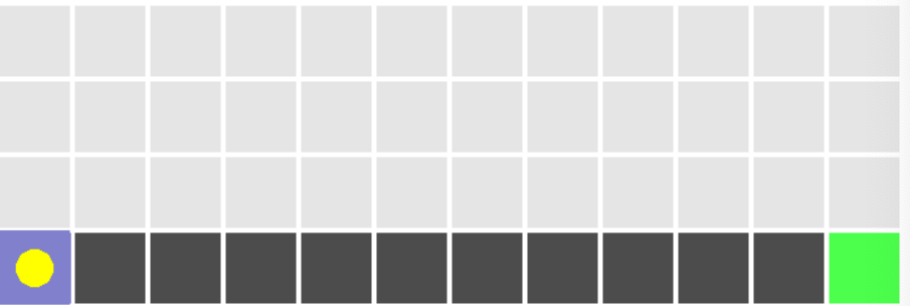
\includegraphics[width=0.4\textwidth]{game1.png}} 
	  \label{fig:oscil}
	\end{figure}
\\The environment is implemented in gym$_$gridworld.py and we won't modify it. The state space and action space are as follows:
\\(1)The state s$_t$ is an integer, which represents the current coordinate (x,y) of the agent, i.e. s$_t$ = x + 12*y. 
\\(2)A discrete variable, where 0,1,2,3 represent move leftward, rightward, upward, downward respectively.
\subsection{Game with Sarsa and Q-learning}
We need to implement agents based on Sarsa and Q-learning algorithms, implement the agents in agent.py and complete the training process in cliff$_$walk$_$sarsa.py and cliff$_$walk$_$qlearning.py respectively. 
\subsubsection{Cliff$_$walk$_$sarsa.py}
In this section, we utilize some parameters to construct the agent, such as learning rate, reward decay $\gamma$, $\epsilon$ value, and $\epsilon$-decay schema.
\subsubsection{Agent.py}
We need to implement $\epsilon$-greedy with $\epsilon$ value decay in the choose$\_$action function and functions given in the template need to be completed. We should keep a balance between exploration and exploitation by tuning $\epsilon$ value carefully. 




\subsection{Result Visualization and Analysis}
 We should visualize the process and the final result according to the following requirement:
\begin{itemize}
    \item Plot the episode reward during the training process.
    \item Plot the $\epsilon$ value during the training process.
    \item Visualize the final paths found by the intelligent agents after training.
\end{itemize}
\subsubsection{Code}
\subsubsubsection{Cliff$_$walk$_$qlearning.py}
\\In the cliff$_$walk$_$qlearning, first, we add some instructions below:
\\1.num$_$observations = env.observation$_$space.n
\\num$_$observations obtain all the states from observation$_$space.
\\2.We initialize epsilon as 1 before for episode
\\3.We add a forloop about episode:
\begin{lstlisting}{language=python}
for episode in range(1000):
    episode_reward = 0;
    s = env.reset();
    env.render();
    episode_epsilons.append(epsilon)
    agent.set_epsilon(epsilon)
\end{lstlisting}
This part is added to renew epsilon after every forloop of iter.
\\4.We add an instruction: epsilon = epsilon*0.95;
\\5.We implement matplotlib.pyplot to draw the picture and the code below:
\begin{lstlisting}{language=python}
import matplotlib.pyplot as plt
plt.figure(1)
plt.plot(episode_rewards)
plt.xlabel('Episode')
plt.ylabel('Episode Rewards')
plt.savefig('/Users/xiaojian_xiang/Projects/AI3606/HW2/QLearning/Cliff_reward_zero.png')
plt.show()

plt.figure(2)
plt.plot(episode_epsilons)
plt.xlabel('Episode')
plt.ylabel('Episode Epsilons')
plt.savefig('/Users/xiaojian_xiang/Projects/AI3606/HW2/QLearning/Cliff_epsilon_zero.png')
plt.show()

print('\ntraining over\n')   

# close the render window after training.
env.close()

##### START CODING HERE #####
\end{lstlisting}
\subsubsubsection{Agent.py}
\\In this part, we added predict function, save function, restore function and set$_$epsilon function in the class QlearningAgent
\\Choose$_$action:
\begin{lstlisting}{language=python}
def choose_action(self, observation):
        """choose action with epsilon-greedy algorithm."""
        if np.random.rand() <= self.epsilon:
            # epsilon randomly choose action
            action = np.random.choice(self.all_actions)
        else:
            # greedily choose action
            action = self.predict(observation)
        return action
\end{lstlisting}
\subsubsubsection{Cliff$_$walk$_$sarsa.py}
\\In this part, in the forloop "for episode in range (1000)", we changed the code below:
\begin{lstlisting}
for episode in range(1000):
    # record the reward in an episode
    episode_reward = 0
    # reset env
    s = env.reset()
    # render env. You can comment all render() to turn off the GUI to accelerate training.
    env.render()
    # agent interacts with the environment
    episode_epsilons.append(epsilon + 0.05)
    agent.set_epsilon(epsilon + 0.05)
    # episode_epsilons.append(epsilon)
    # agent.set_epsilon(epsilon)
    # Set epsilon = epsilon(k-1) * 0.95
    #agent.set_lr(learning_rate)
    a = agent.choose_action(s)
\end{lstlisting}

\subsubsection{Result Visualization}
\subsubsubsection{Epsilon reward during the training process}
\begin{figure}[H]
	  \centering
	  \subfloat[Epsilon$_$reward]{\label{fig:Per6A}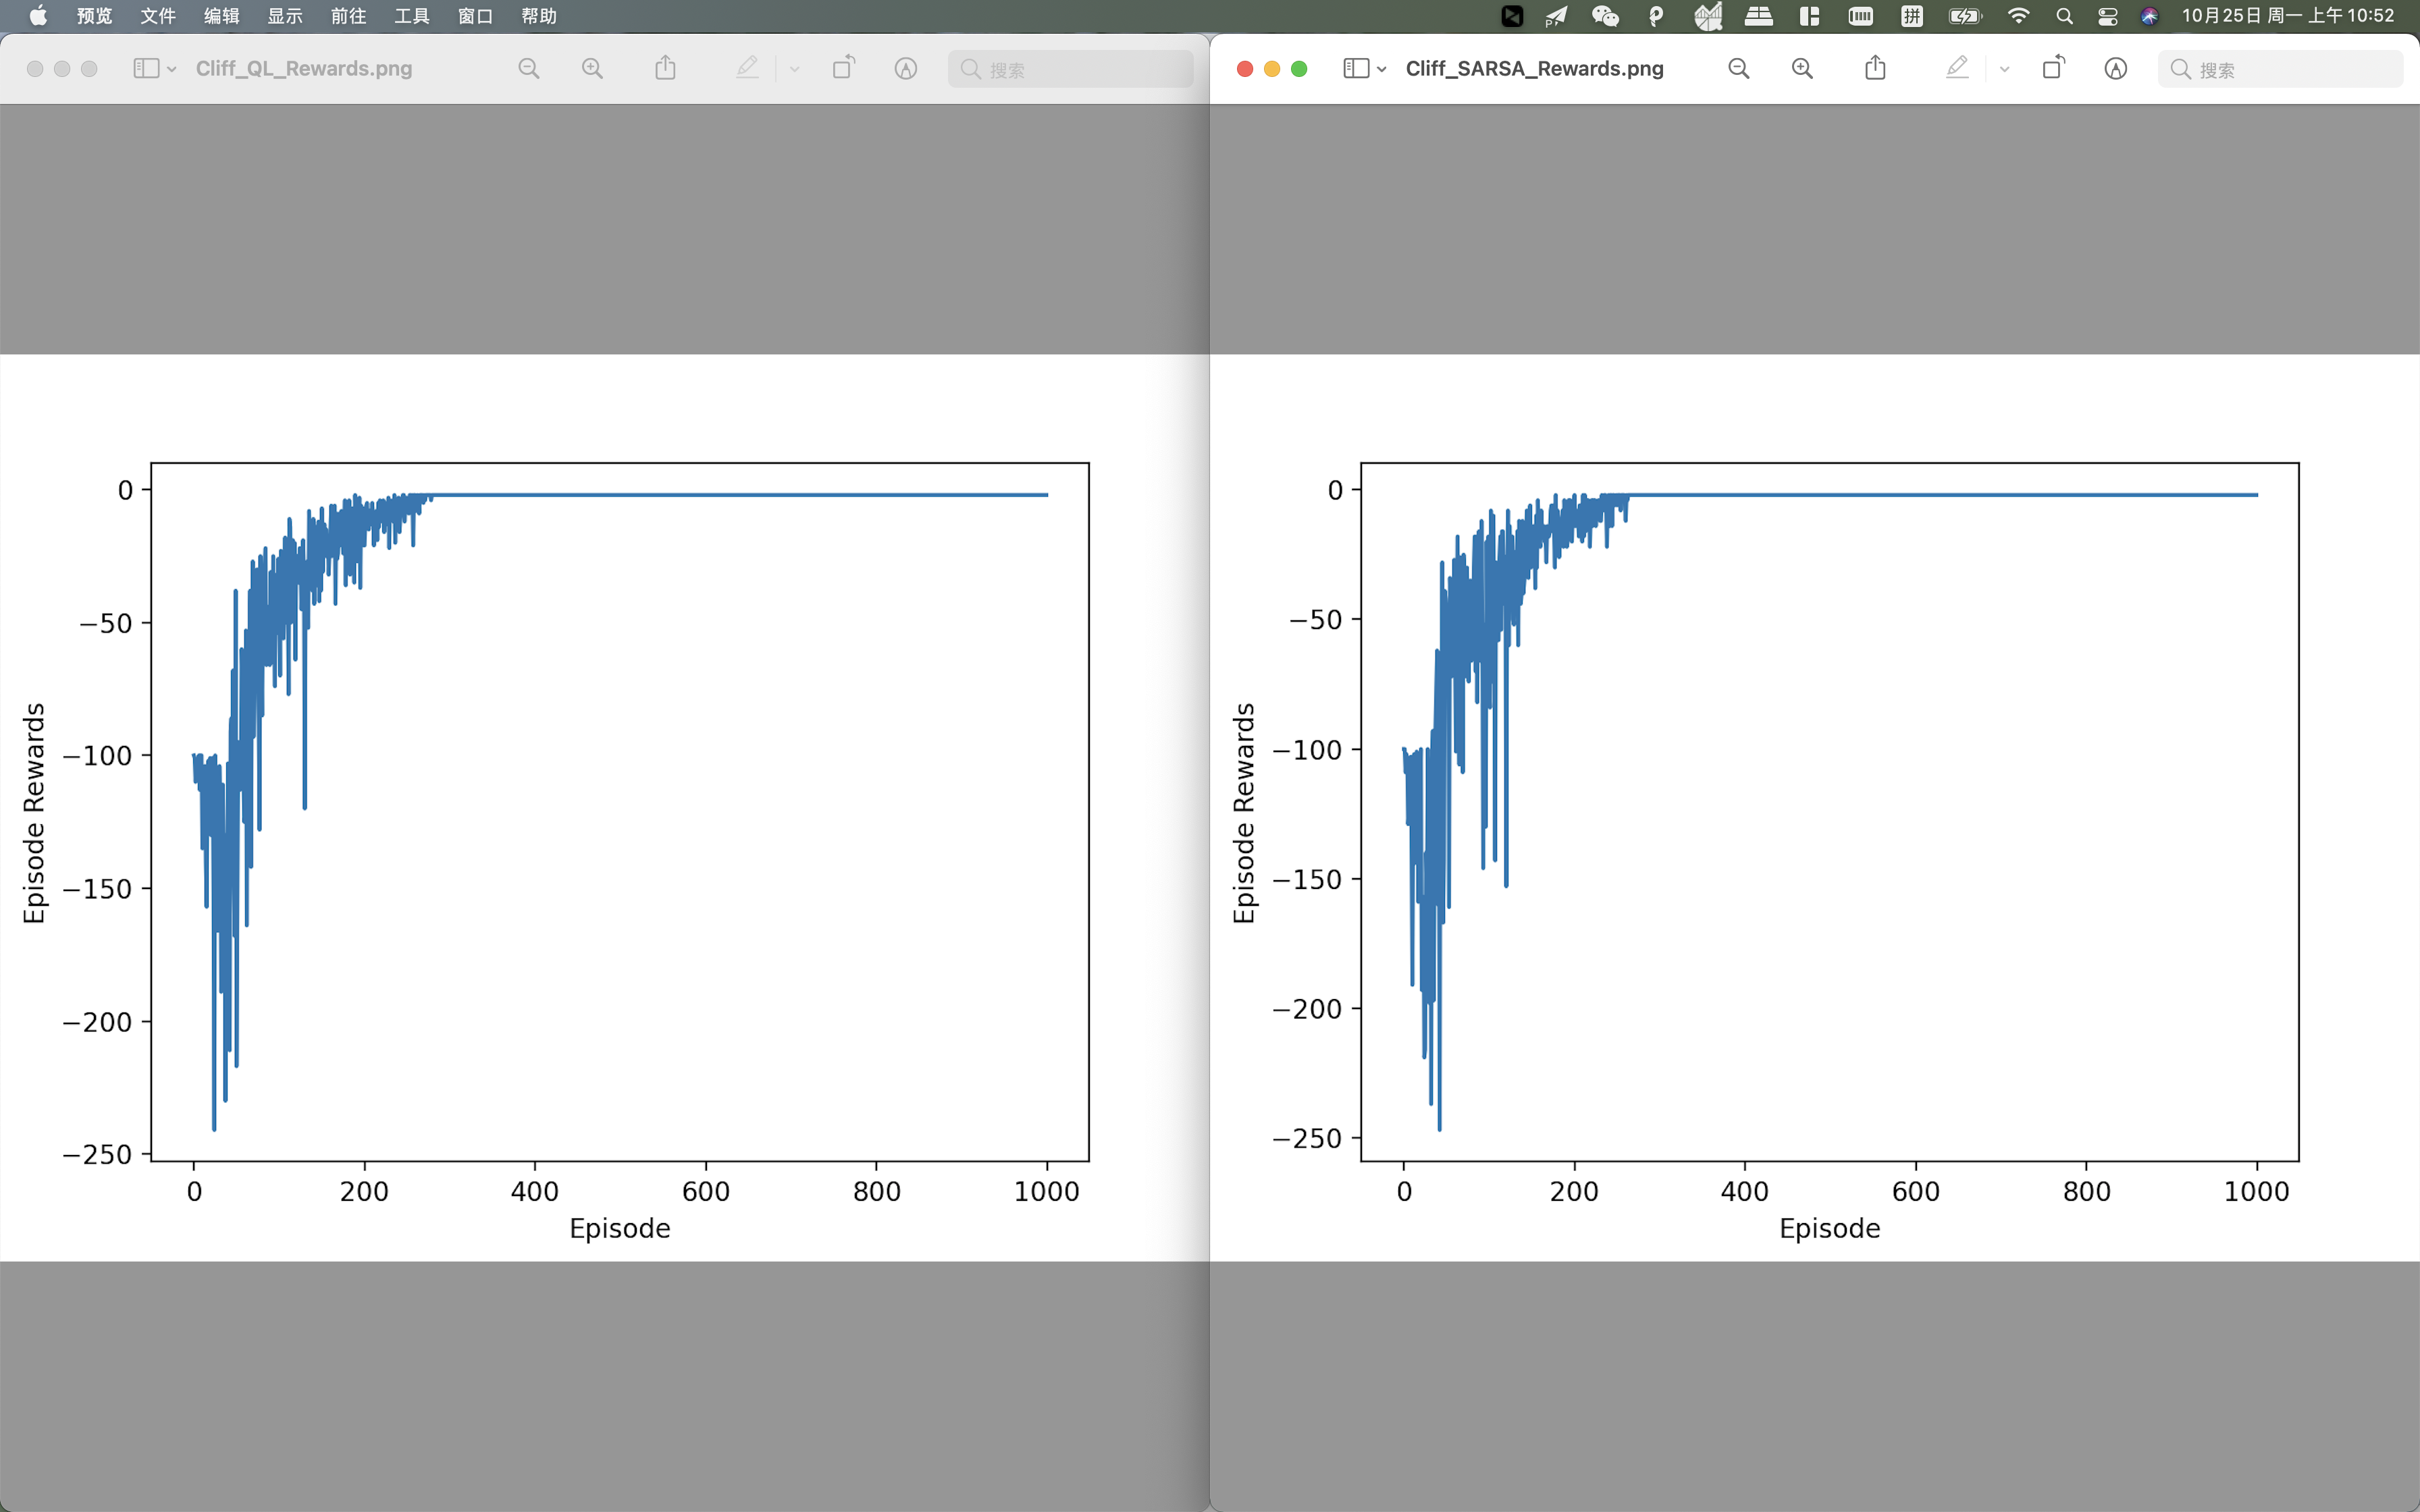
\includegraphics[width=0.4\textwidth]{epsilon_reward.png}} 
	  \label{fig:oscil}
	\end{figure}
The left picture is qlearning and the right is sarsa.
\subsubsubsection{the $epsilon$ value during the training process}
First, we try to make $epsilon$ converge to 0 but we found that the paths we get through using qlearning and sarsa are the same. So we make $epsilon$ converge to 0.1 then we found paths became different. Cause during the training process if we let epsilon converge to 0, then the path of sarsa algorithm will converge to the optimal path, the same as qlearning. Therefore, we obtain two different results and get four pictures.
\begin{figure}[H]
	  \centering
	  \subfloat[Cliff$_$epsilon$_$zero$_$qlearning]{\label{fig:Per6A}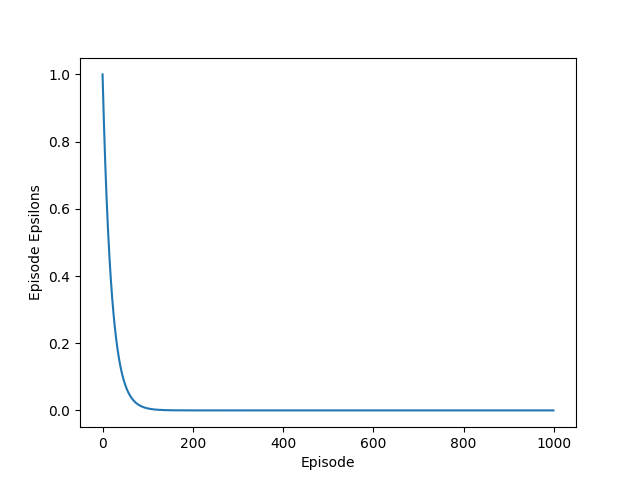
\includegraphics[width=0.4\textwidth]{Cliff_epsilon_zero_qlearning.png}} 
	  \label{fig:oscil}
	\end{figure}
\begin{figure}[H]
	  \centering
	  \subfloat[Cliff$_$epsilon$_$nozero$_$qlearning]{\label{fig:Per6A}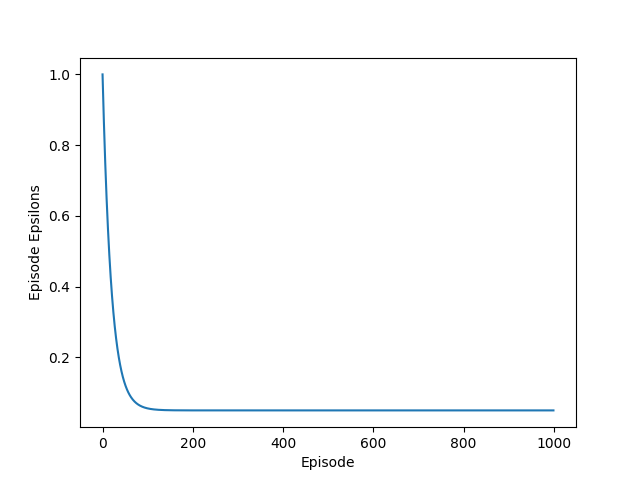
\includegraphics[width=0.4\textwidth]{Cliff_epsilon_nozero_qlearning.png}} 
	  \label{fig:oscil}
	\end{figure}
\begin{figure}[H]
	  \centering
	  \subfloat[Cliff$_$epsilon$_$zero$_$sarsa]{\label{fig:Per6A}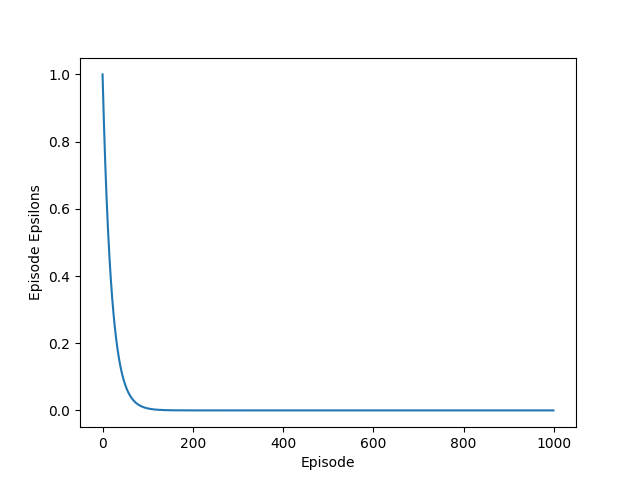
\includegraphics[width=0.4\textwidth]{Cliff_epsilon_zero_sarsa.png}} 
	  \label{fig:oscil}
	\end{figure}
\begin{figure}[H]
	  \centering
	  \subfloat[Cliff$_$epsilon$_$nozero$_$sarsa]{\label{fig:Per6A}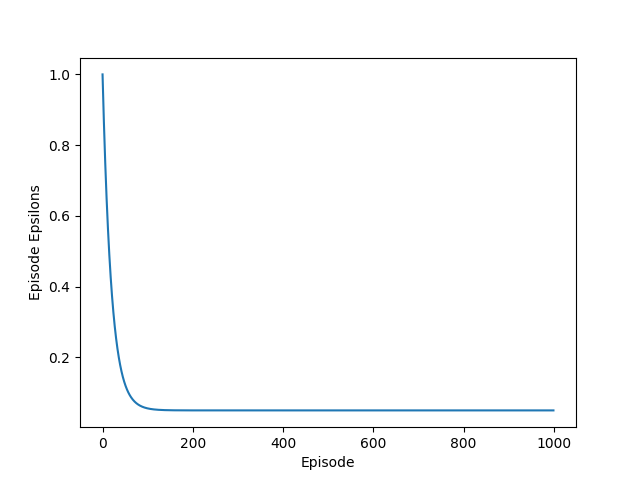
\includegraphics[width=0.4\textwidth]{Cliff_epsilon_nozero_sarsa.png}} 
	  \label{fig:oscil}
	\end{figure}



\subsubsubsection{Paths}
\\First we set the rule that when we reach the purple floor then we turn left, reach the blue floor then we turn right, reach the green floor then we turn up and turn down when we reach the yellow floor.
\begin{figure}[H]
\centering
	  \subfloat[qlearning$_$way]{\label{fig:Per6A}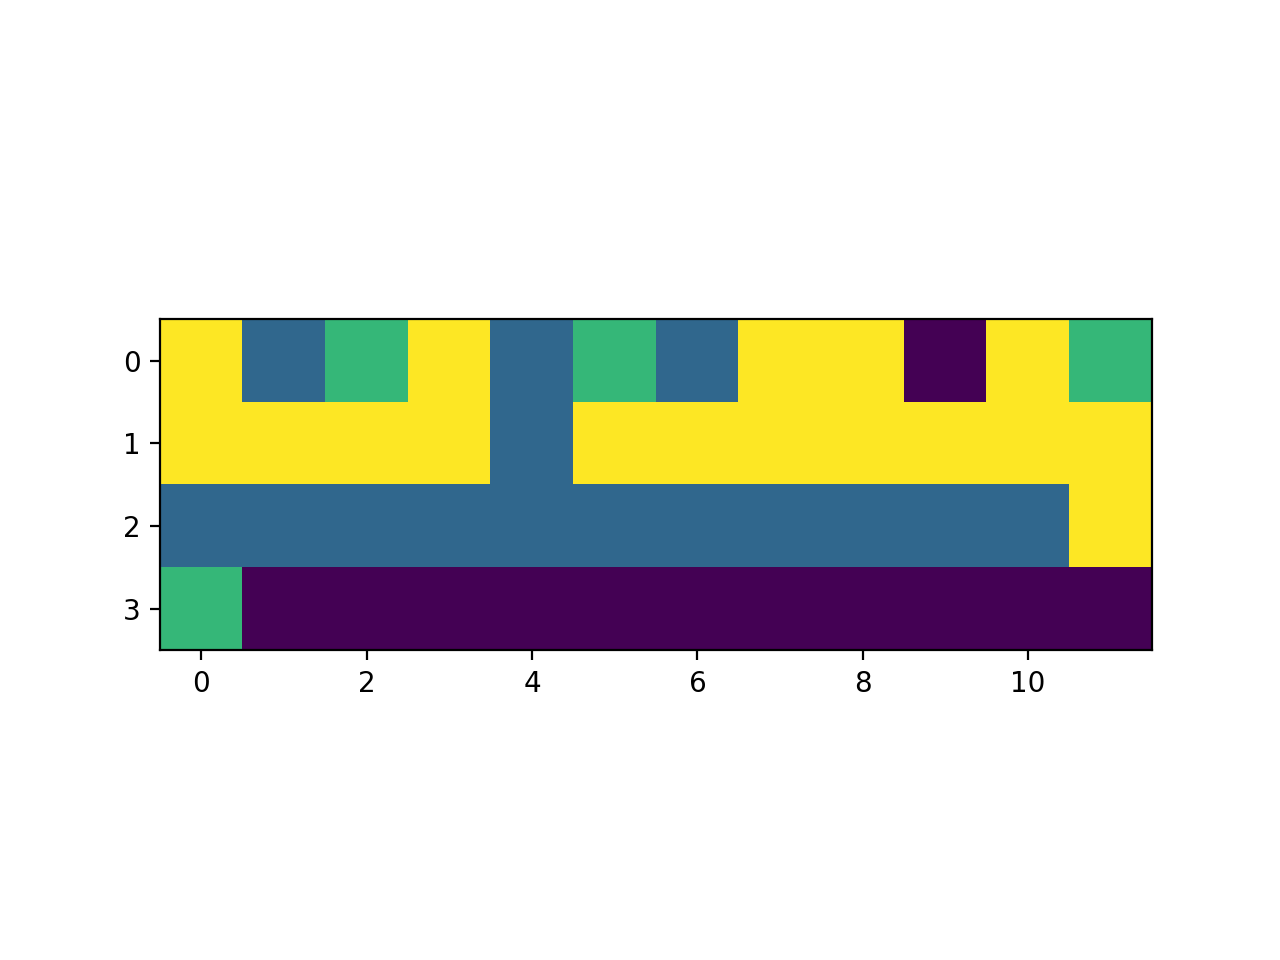
\includegraphics[width=0.4\textwidth]{qlearning_way.png}} 
	 

	  \subfloat[sarsa$_$zero$_$way]{\label{fig:Per6A}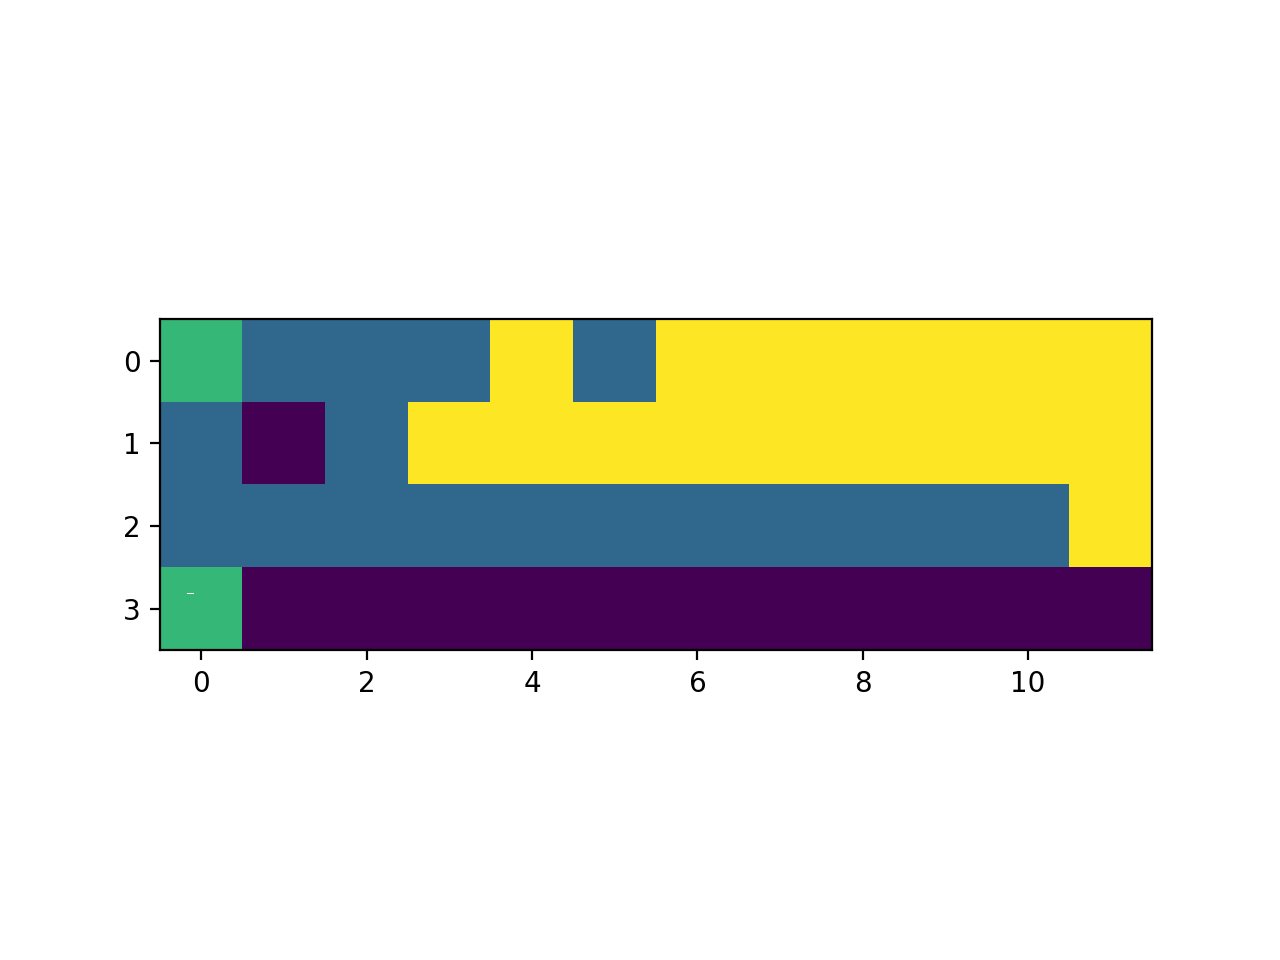
\includegraphics[width=0.4\textwidth]{sarsa_zero_way.png}} 
	  \label{fig:oscil}
	\end{figure}
From the two pictures above, we can know that if we set the epsilon converge to 0, the paths we get are the same. However, if we set the epsilon converge to 0.1, then we get a different path below.
\begin{figure}[H]
	  \centering
	  \subfloat[sarsa$_$nozero$_$way]{\label{fig:Per6A}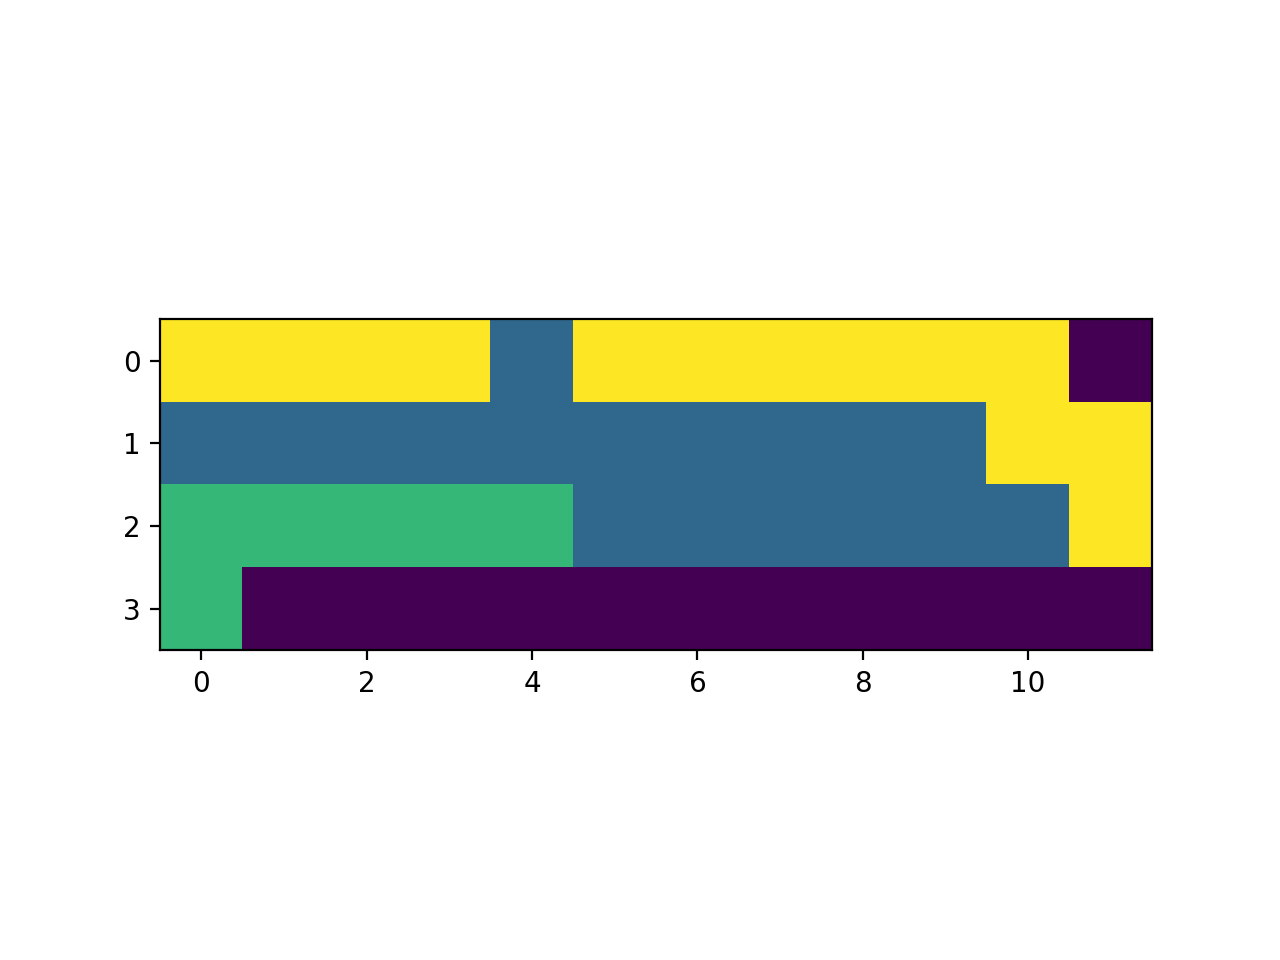
\includegraphics[width=0.4\textwidth]{sarsa_nozero_way.png}} 
	   
	  \label{fig:oscil}
	\end{figure}

\subsubsection{Result Analysis}
\subsubsubsection{Differences between Sarsa and Qlearning}
\\The only difference between Sarsa and Qlearning is the way of updating the value of q.
\\For Q-learning, in the state s$_t$, according to the $epsilon$-greedy, perform the action A$_t$ and reach the state S$_{t+1}$. And in the state S$_{t+1}$, choose the largest action Q(S$_{t+1}$,a). In the state S$_{t+1}$, we choose the same strategy to perform actions.
\\For Sarsa, in the state s$_t$, according the $epsilon$-greedy strategy, perform the action A$_t$ and reach the state S$_{t+1}$, now the way of updating (S$_t$,a) is still the $epsilon$-greedy and really choose (S$_{t+1}$,a).
\\For two algorithms, both are choosing $epsilon$-greedy strategy, the differences are the way of updating the value of Q in the Q-learning is greedy strategy-choose the largest Q(S$_{t+1}$,a), but the way of updating the value of Q in the Sarsa is still the $epsilon$-greedy.



\section{Reinforcement Learning in the Sokoban Game}
In this part, we should implement intelligent agents to play the Sokoban game utilizing Sarsa, Q-learning and dyna-Q algorithms. Therefore, we will have a deeper understanding on the model-based RL algorithms and the explore-exploit dilemma.
\subsection{Introduction of game rule}
As shown in the picture, the game is a transportation puzzle, where the player has to push all boxes in the room on the storage targets. The possibility of making irreversible mistakes makes this game a bit challenging for RL agents.
\begin{figure}[H]
	  \centering
	  \subfloat[game2]{\label{fig:Per6A}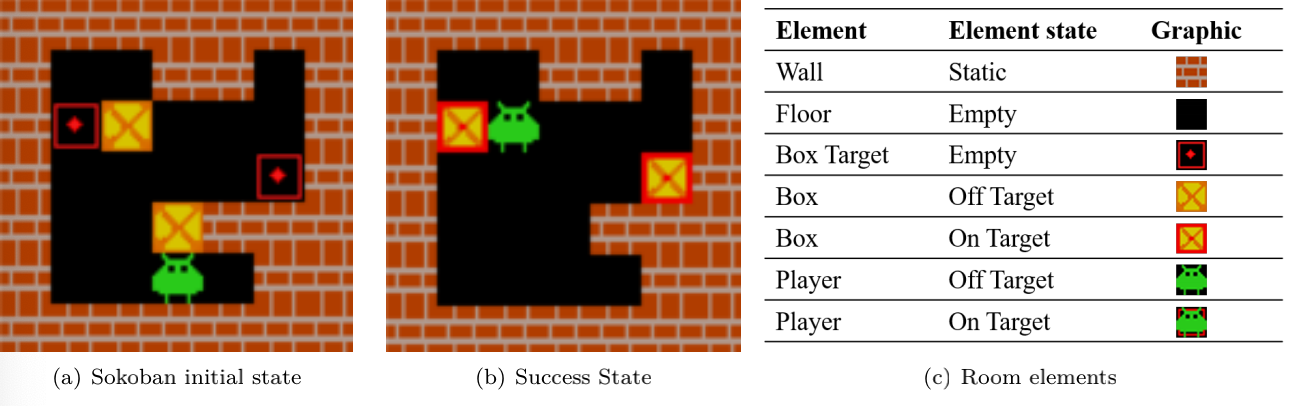
\includegraphics[width=0.4\textwidth]{game2.png}} 
	   
	  \label{fig:oscil}
	\end{figure}

\\In this task, a 7*7 room with two boxes is utilized, as illustrated in Fig.2(a). The environment utilized in this task is static, i.e. the room settings including box coordinates, target position, and agent positions are the same after each reset. In this game, we can move upward, downward, leftward and rightward. Pushing two boxes onto the targets gives a reward +10; Pushing one box on box on a target gives a reward +1, while pushing a box off the target gives -1. In addition, a reward of -0.1 is given for each step as living cost. the game terminates when two boxes are pushed onto the target, or 100 steps are exhausted before success.
\\State(Array): The state s$_t$ is an array composed of 6 integers, where the first two integers represent current coordinate of the agent, and the last four integers represent current coordinates of two boxes in the room.
\\Action(Integer): A discrete variable and 0, 1, 2, 3 represent move upward, downward, leftward, rightward respectively.
\subcection{Game with RL algorithms}
We should solve this task utilizing Sarsa, Q-learing, and Dyna-Q algorithms repectively. We should implement the intelligent agents in agent.py and complete the training process in sokoban$_$sarsa.py, sokoban$_$qlearning.py and sokoban$_$dynaq.py respectively. Actually, Sarsa and Q-learning agents implemented in Section First part can be utilized for this task.
\subsection{Result Visualization and Analysis}
\subsubsection{Result Visualization} We should visualize the training process and the final result according to the following requirements:
\begin{itemize}
    \item Plot the episode rewards during the training process.
    \item Plot the $epsilon$ value during the training process.
    \item Visualize the final result of the three agents and we ought to record videos of the final result. 
\end{itemize}
\subsubsubsection{The episode reward during the training process}
\begin{figure}[H]
	  \centering
	  \subfloat[SO$_$ql$_$reward$_$zero]{\label{fig:Per6A}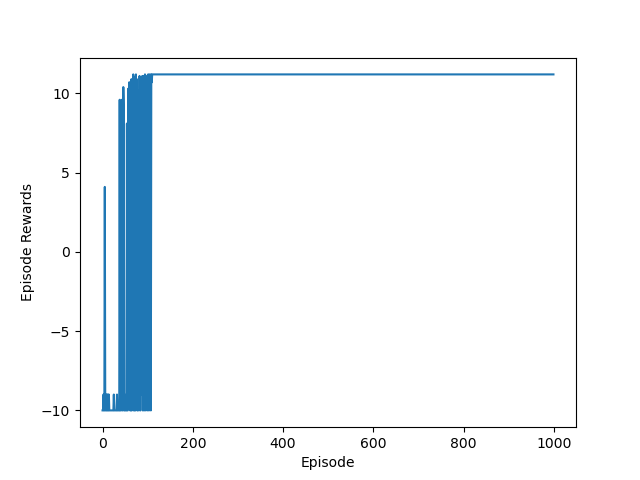
\includegraphics[width=0.4\textwidth]{SO_ql_reward_zero.png}} 
	   
	  \label{fig:oscil}
	\end{figure}
\begin{figure}[H]
	  \centering
	  \subfloat[SO$_$ql$_$reward$_$nozero]{\label{fig:Per6A}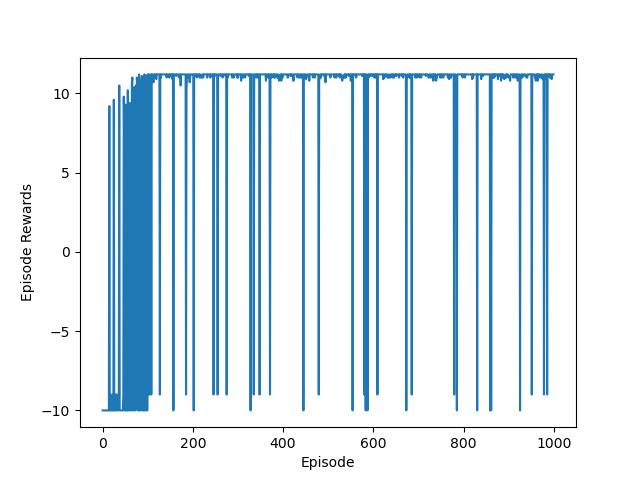
\includegraphics[width=0.4\textwidth]{SO_ql_reward_nozero.png}} 
	   
	  \label{fig:oscil}
	\end{figure}
\begin{figure}[H]
	  \centering
	  \subfloat[SO$_$sa$_$reward$_$zero]{\label{fig:Per6A}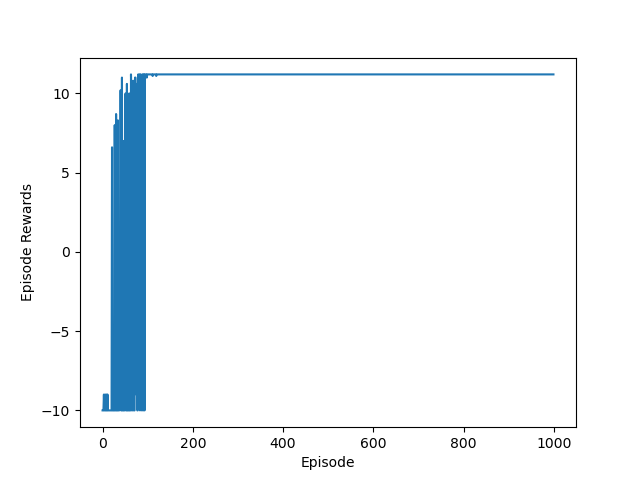
\includegraphics[width=0.4\textwidth]{SO_sa_reward_zero.png}} 
	   
	  \label{fig:oscil}
	\end{figure}
\begin{figure}[H]
	  \centering
	  \subfloat[SO$_$sa$_$reward$_$nozero]{\label{fig:Per6A}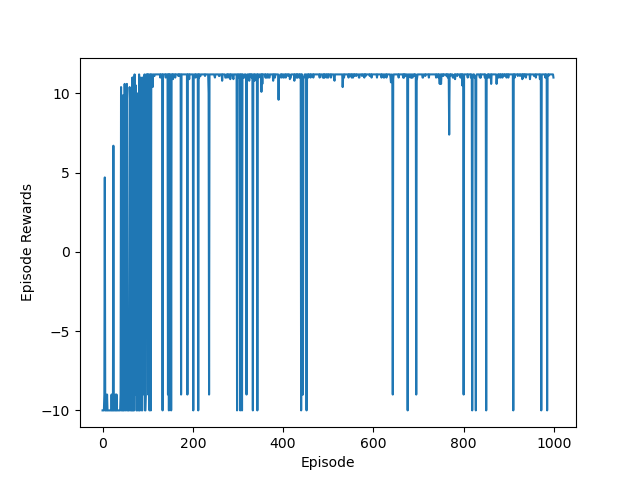
\includegraphics[width=0.4\textwidth]{SO_sa_reward_nozero.png}} 
	   
	  \label{fig:oscil}
	\end{figure}
\subsubsubsection{The $epsilon$ value during the training process}
\begin{figure}[H]
	  \centering
	  \subfloat[SO$_$ql$_$epsilon$_$zero]{\label{fig:Per6A}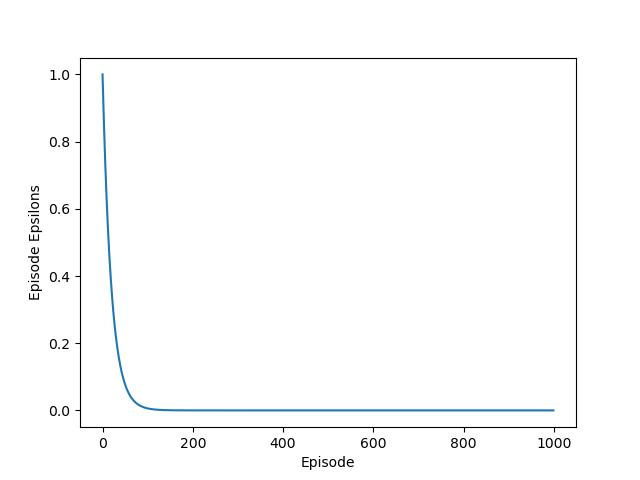
\includegraphics[width=0.4\textwidth]{SO_ql_epsilon_zero.png}} 
	   
	  \label{fig:oscil}
	\end{figure}
	\begin{figure}[H]
	  \centering
	  \subfloat[SO$_$ql$_$epsilon$_$nozero]{\label{fig:Per6A}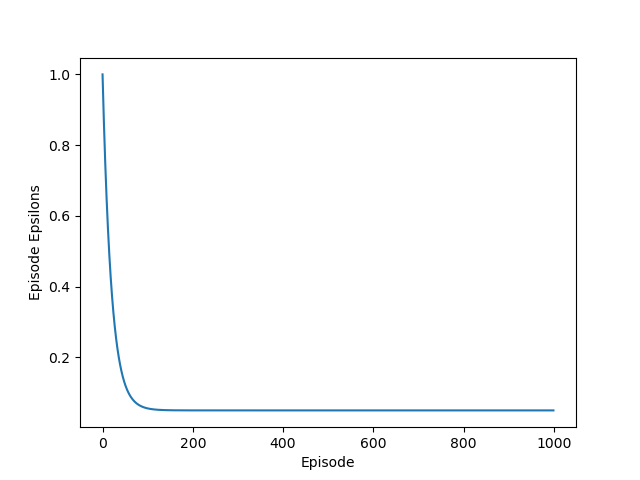
\includegraphics[width=0.4\textwidth]{SO_ql_epsilon_nozero.png}} 
	   
	  \label{fig:oscil}
	\end{figure}
	\begin{figure}[H]
	  \centering
	  \subfloat[SO$_$sa$_$epsilon$_$zero]{\label{fig:Per6A}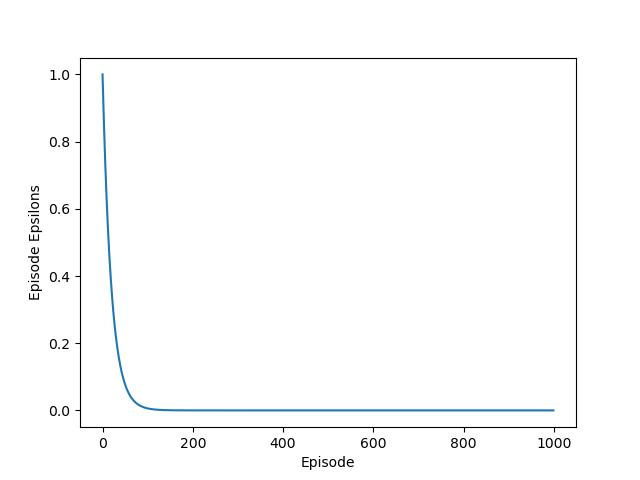
\includegraphics[width=0.4\textwidth]{SO_sa_epsilon_zero.png}} 
	   
	  \label{fig:oscil}
	\end{figure}	
		\begin{figure}[H]
	  \centering
	  \subfloat[SO$_$sa$_$epsilon$_$nozero]{\label{fig:Per6A}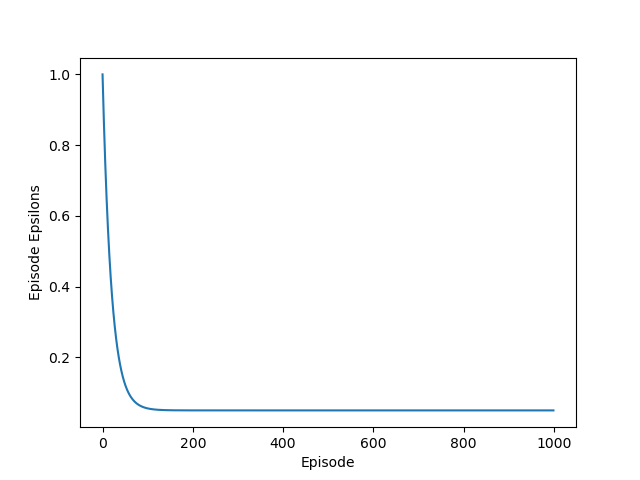
\includegraphics[width=0.4\textwidth]{SO_sa_epsilon_nozero.png}} 
	   
	  \label{fig:oscil}
	\end{figure}
	
\\From the four pictures above, we can see that the epsilon converge to 0 and 0.1. 
\\Then we applied dyna-q algorithm and get the results below:
\begin{figure}[H]
	  \centering
	  \subfloat[SO$_$dynaq$_$epsilon$_$zero]{\label{fig:Per6A}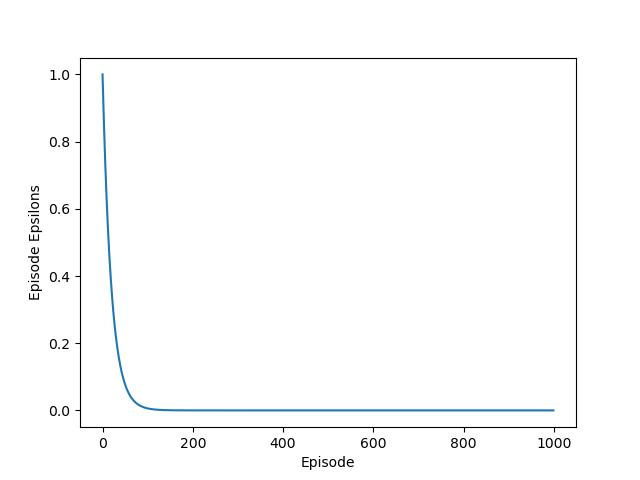
\includegraphics[width=0.4\textwidth]{SO_dynaq_epsilon_zero.png}} 
	   
	  \label{fig:oscil}
	\end{figure}
	\begin{figure}[H]
	  \centering
	  \subfloat[SO$_$dynaq$_$epsilon$_$nozero]{\label{fig:Per6A}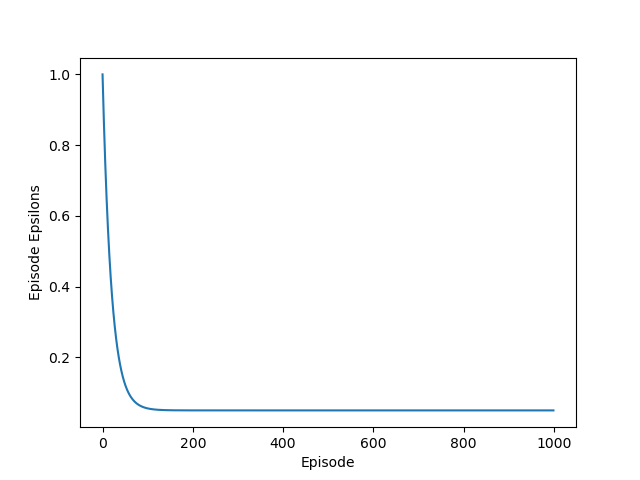
\includegraphics[width=0.4\textwidth]{SO_dynaq_epsilon_nozero.png}} 
	   
	  \label{fig:oscil}
	\end{figure}
	\begin{figure}[H]
	  \centering
	  \subfloat[SO$_$dynaq$_$reward$_$zero]{\label{fig:Per6A}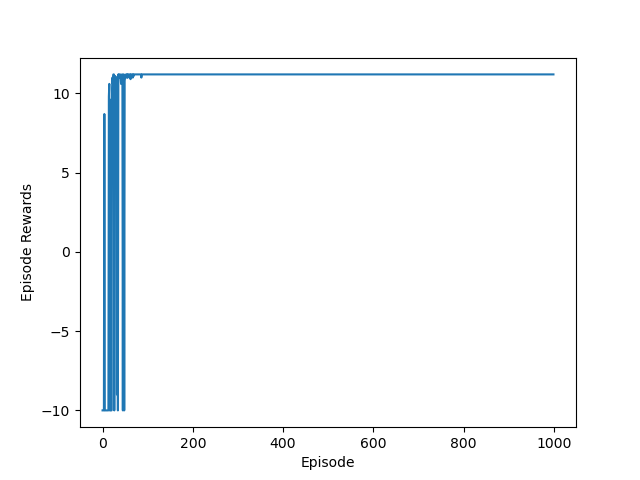
\includegraphics[width=0.4\textwidth]{SO_dynaq_reward_zero.png}} 
	   
	  \label{fig:oscil}
	\end{figure}	
		\begin{figure}[H]
	  \centering
	  \subfloat[SO$_$dynaq$_$reward$_$nozero]{\label{fig:Per6A}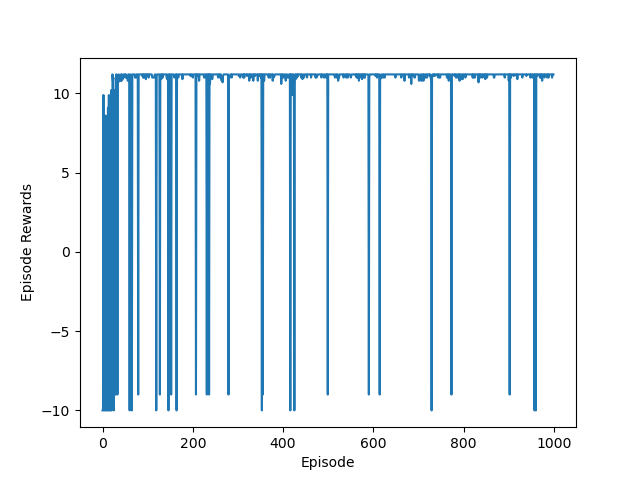
\includegraphics[width=0.4\textwidth]{SO_dynaq_reward_nozero.png}} 
	   
	  \label{fig:oscil}
	\end{figure}


\subsubsubsection{The final results of three agents}
The results are recorded videos in the file list.
And from the videos, we can know that the paths are different through different algorithms.

\section{Explore-Exploit Dilemma}
We have found the importance of exploration-exploitation dilemma in the Reinforcement Learning through previous experiments. So in this section, we should analyze the influence of different exploration schemes on the learning speed and result.
\begin{itemize}
    \item Conduct experiments in the Sokoban environment utilizing any one RL algorithm with different $epsilon$ values and $epsilon$-decay schemes. Try to summarize the relationship between different exploration schemes and learning speeds/results.
    \item Actually, there exists lots of other exploration strategies except $epsilon$-greedy. We can find and learn one new exploration method, such as Upper Confidence Bound(UCB)
    \item(Bonus)Implement the exploration strategy we have found in the Sokoban environment. We can add new agent class in the agent.py and the corresponding training process should be implemented in sokoban$_$new$_$exploration.py.
\end{itemize}
\subsection{Result Visualization and Analysis}
About this algorithm, we spent a lot of time hoping to finish it.
\subsubsection{Result Visualization}
		\begin{figure}[H]
	  \centering
	  \subfloat[SO$_$reward$_$zero]{\label{fig:Per6A}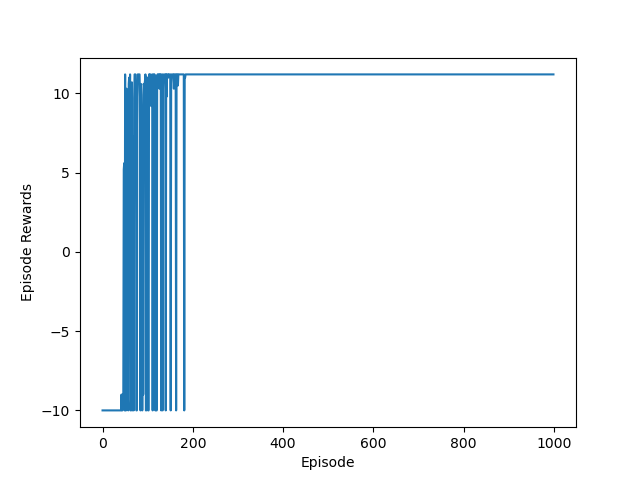
\includegraphics[width=0.4\textwidth]{SO_reward_zero.png}} 
	   
	  \label{fig:oscil}
	\end{figure}
		\begin{figure}[H]
	  \centering
	  \subfloat[SO$_$epsilon$_$zero]{\label{fig:Per6A}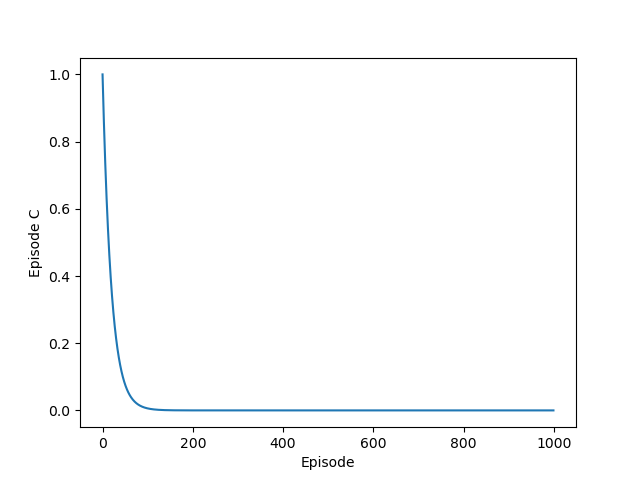
\includegraphics[width=0.4\textwidth]{SO_epsilon_zero.png}} 
	   
	  \label{fig:oscil}
	\end{figure}
\subsubsection{Result Analysis}
There are some advantages of Upper confidence Bound over other algorithms. First, it makes a good banlance between exploitation and exploration.Second, this exploration is an optimization exploration and the action of each exploration is certain.Third, it is proved that it can converge to the optimal strategy in finite time. In addition, it performs better than Q-learning algorithm, Sarsa algorithm and Dynaq algorithm.What's more, from the pictures above, we can see that it has a faster convergence and we have provided comparison diagram in the files.
\section{Discussion \& Conclusion}
\subsection{Submission File List}
\begin{itemize}
    \item agent.py:Implementation of RL agents;
    \item cliff$_$walk$_$sarsa.py:train Sarsa in Cliff$_$walking environment.
    \item cliff$_$walk$_$qlearning.py:train Q-learning in Cliff-walking environment.
    \item sokoban$_$qlearning.py:train Q-Learing in Sokoban environment.
    \item sokoban$_$sarsa.py:train Sarsa in Sokoban environment.
    \item sokoban$_$dynanq.py: train Dyna-Q in Sokoban environment.
    \item sokoban$_$new$_$exploration.py:(Optional, Bonus)train RL agent with new exploration method in Sokoban environment.
    \item videos(floder): Demo videos recorded.
    \item gym$_$sokoban(folder):Sokoban game environment.
    \item gym$_$gridworld.py: Cliff-Walking game environment.
    \item All the pictures and videos during the experiment are listed in the files.
\end{itemize}

\subsection{Conclusion}
In this homework, we applied qlearning and sarsa algorithm to run two games: Cliff$_$walking and Sokoban and we succeeded to perform the algorithms. During the process, we observed the change of episode reward and $epsilon$ value. At last, we applied Upper Confidence Bound(UCB) to optimize the results we got before. In conclusion, we obtain a lot of knowledge about reinforcement learning and had a keen interest in this and we hope we can learn more about reinforcement learning in the following learning process.


\end{document} % DONE WITH DOCUMENT!


%%%%%%%%%%
PERSONAL FAVORITE LAB WRITE-UP STRUCTURE
%%%%%%%%%%
\section{Introduction}
	% No Text Here
	\subsection{Purpose}
		% Lab objective
	\subsection{Equipment}
		% Any and all equipment used (specific!)
	\subsection{Procedure}
		% Overview of the procedure taken (not-so-specific!)
\newpage
\section{Schematic Diagrams}
	% Any schematics, screenshots, block
   % diagrams used.  Possibly photos or
	% images could go here as well.
\newpage
\section{Experiment Data}
	% Depending on lab, program code would be
	% included here without the Estimated and
	% Actual Results.
	\subsection{Estimated Results}
		% Calculated. What it should be.
	\subsection{Actual Results}
		% Measured.  What it actually was.
\newpage
\section{Discussion \& Conclusion}
	% 3 Paragraphs:
		% Restate the objective of the lab
		% Discuss personal trials, errors, and difficulties
		% Conclude the lab


%%%%%%%%%%%%%%%%
COMMON COMMANDS:
%%%%%%%%%%%%%%%%
% IMAGES
begin{figure}[H]
   \begin{center}
      \includegraphics[width=0.6\textwidth]{RTL_SCHEM.png}
   \end{center}
\caption{A screenshot of the RTL Schematics produced from the Verilog code.}
\label{RTL}
\end{figure}

% SUBFIGURES IMAGES
\begin{figure}[H]
  \centering
  \subfloat[LED4 Period]{\label{fig:Per4}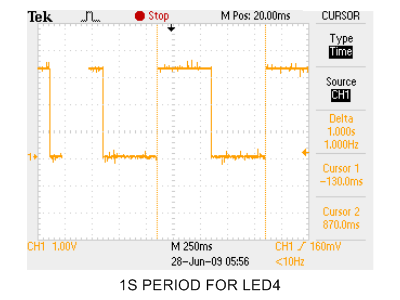
\includegraphics[width=0.4\textwidth]{period_led4.png}} \\
  \subfloat[LED5 Period]{\label{fig:Per5}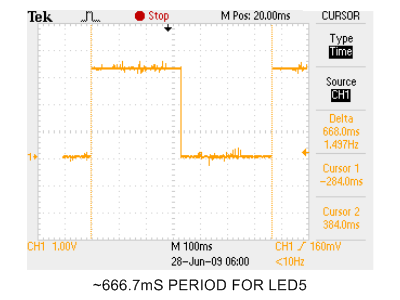
\includegraphics[width=0.4\textwidth]{period_led5.png}}
  \subfloat[LED6 Period]{\label{fig:Per6}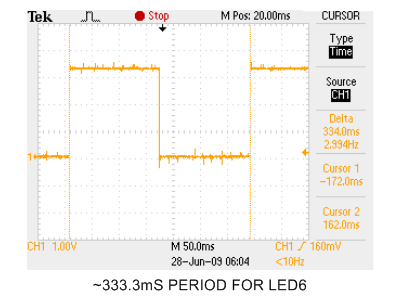
\includegraphics[width=0.4\textwidth]{period_led6.png}}
  \caption{Period of LED blink rate captured by osciliscope.}
  \label{fig:oscil}
\end{figure}

% INSERT SOURCE CODE
\lstset{language=Verilog, tabsize=3, backgroundcolor=\color{mygrey}, basicstyle=\small, commentstyle=\color{BrickRed}}
\lstinputlisting{MODULE.v}

% TEXT TABLE
\begin{table}
\begin{center}
\begin{tabular}{|l|c|c|l|}
	x & x & x & x \\ \hline
	x & x & x & x \\
	x & x & x & x \\ \hline
\end{tabular}
\caption{Caption}
\label{label}
\end{center}
\end{table}

% MATHMATICAL ENVIRONMENT
$ 8 = 2 \times 4 $

% CENTERED FORMULA
\[  \]

% NUMBERED EQUATION
\begin{equation}
	
\end{equation}

% ARRAY OF EQUATIONS (The splat supresses the numbering)
\begin{align*}
	
\end{align*}

% NUMBERED ARRAY OF EQUATIONS
\begin{align}
	
\end{align}

% ACCENTS
\dot{x} % dot
\ddot{x} % double dot
\bar{x} % bar
\tilde{x} % tilde
\vec{x} % vector
\hat{x} % hat
\acute{x} % acute
\grave{x} % grave
\breve{x} % breve
\check{x} % dot (cowboy hat)

% FONTS
\mathrm{text} % roman
\mathsf{text} % sans serif
\mathtt{text} % Typewriter
\mathbb{text} % Blackboard bold
\mathcal{text} % Caligraphy
\mathfrak{text} % Fraktur

\textbf{text} % bold
\textit{text} % italic
\textsl{text} % slanted
\textsc{text} % small caps
\texttt{text} % typewriter
\underline{text} % underline
\emph{text} % emphasized

\begin{tiny}text\end{tiny} % Tiny
\begin{scriptsize}text\end{scriptsize} % Script Size
\begin{footnotesize}text\end{footnotesize} % Footnote Size
\begin{small}text\end{small} % Small
\begin{normalsize}text\end{normalsize} % Normal Size
\begin{large}text\end{large} % Large
\begin{Large}text\end{Large} % Larger
\begin{LARGE}text\end{LARGE} % Very Large
\begin{huge}text\end{huge}   % Huge
\begin{Huge}text\end{Huge}   % Very Huge


% GENERATE TABLE OF CONTENTS AND/OR TABLE OF FIGURES
% These seem to have some issues with the "revtex4" document class.  To use, change
% the very first line of this document to "article" like this:
% \documentclass[aps,letterpaper,10pt]{article}
\tableofcontents
\listoffigures
\listoftables

% INCLUDE A HYPERLINK OR URL
\url{http://www.derekhildreth.com}
\href{http://www.derekhildreth.com}{Derek Hildreth's Website}

% FOR MORE, REFER TO THE "LINUX CHEAT SHEET.PDF" FILE INCLUDED!
